\section{Hubo2 Plus}
Hubo2 Plus is a 130 $cm$ (4' 3'') tall, 42 $kg$ (93 $lb$) full-size humanoid robot commonly refered to as Hubo.  
It was designed and constructed by Prof Jun-Ho Oh at the Hubo Lab in the Korean Advanced Institute of Science and Technology (KAIST)\cite{hubo-first}.
Hubo is anthropomorphic to a human meaning it has 2 arms, 2 legs and a head.
There are 6 degreese of freedom (DOF) in each leg, 6 in each arm, 5 in each hand, 3 in the neck, and 1 in the waist; all totalling 38 DOF.
All joints of the major joints are high gain PD position controlled with the exception of the fingers.
The fingers are open-loop PWM controlled.
The sensing capiability consists of a three axis force-torque (FT) sensor on each leg between the end of the ankle and the foot as well as between where the arm connects to the hand.
Additionally it has an inertial measurement unit (IMU) at the center of mass and accelerometers on each foot.
The reference commands for all of the joints are sent from the primary control computer (x86) to the individual motor controllers via two Controller Area Network (CAN) buses.
There are currently eight Hubo's functioning in the United States as of December 2012.
Four reside at Drexel University and one at Georgia Tech, Perdue, Ohio State and MIT.
Jaemi Hubo is the oldest of the Hubos in America and has been at the Drexel Autonomous Systems Lab\footnote{Drexel Autonomous Systems Lab: http://dasl.mem.drexel.edu/} (DASL) since 2008\cite{jaemiHuboSRM}.
Fig.~\ref{fig:hubo} shows the major dimensions of Hubo.

\begin{figure}[thpb]
  \centering
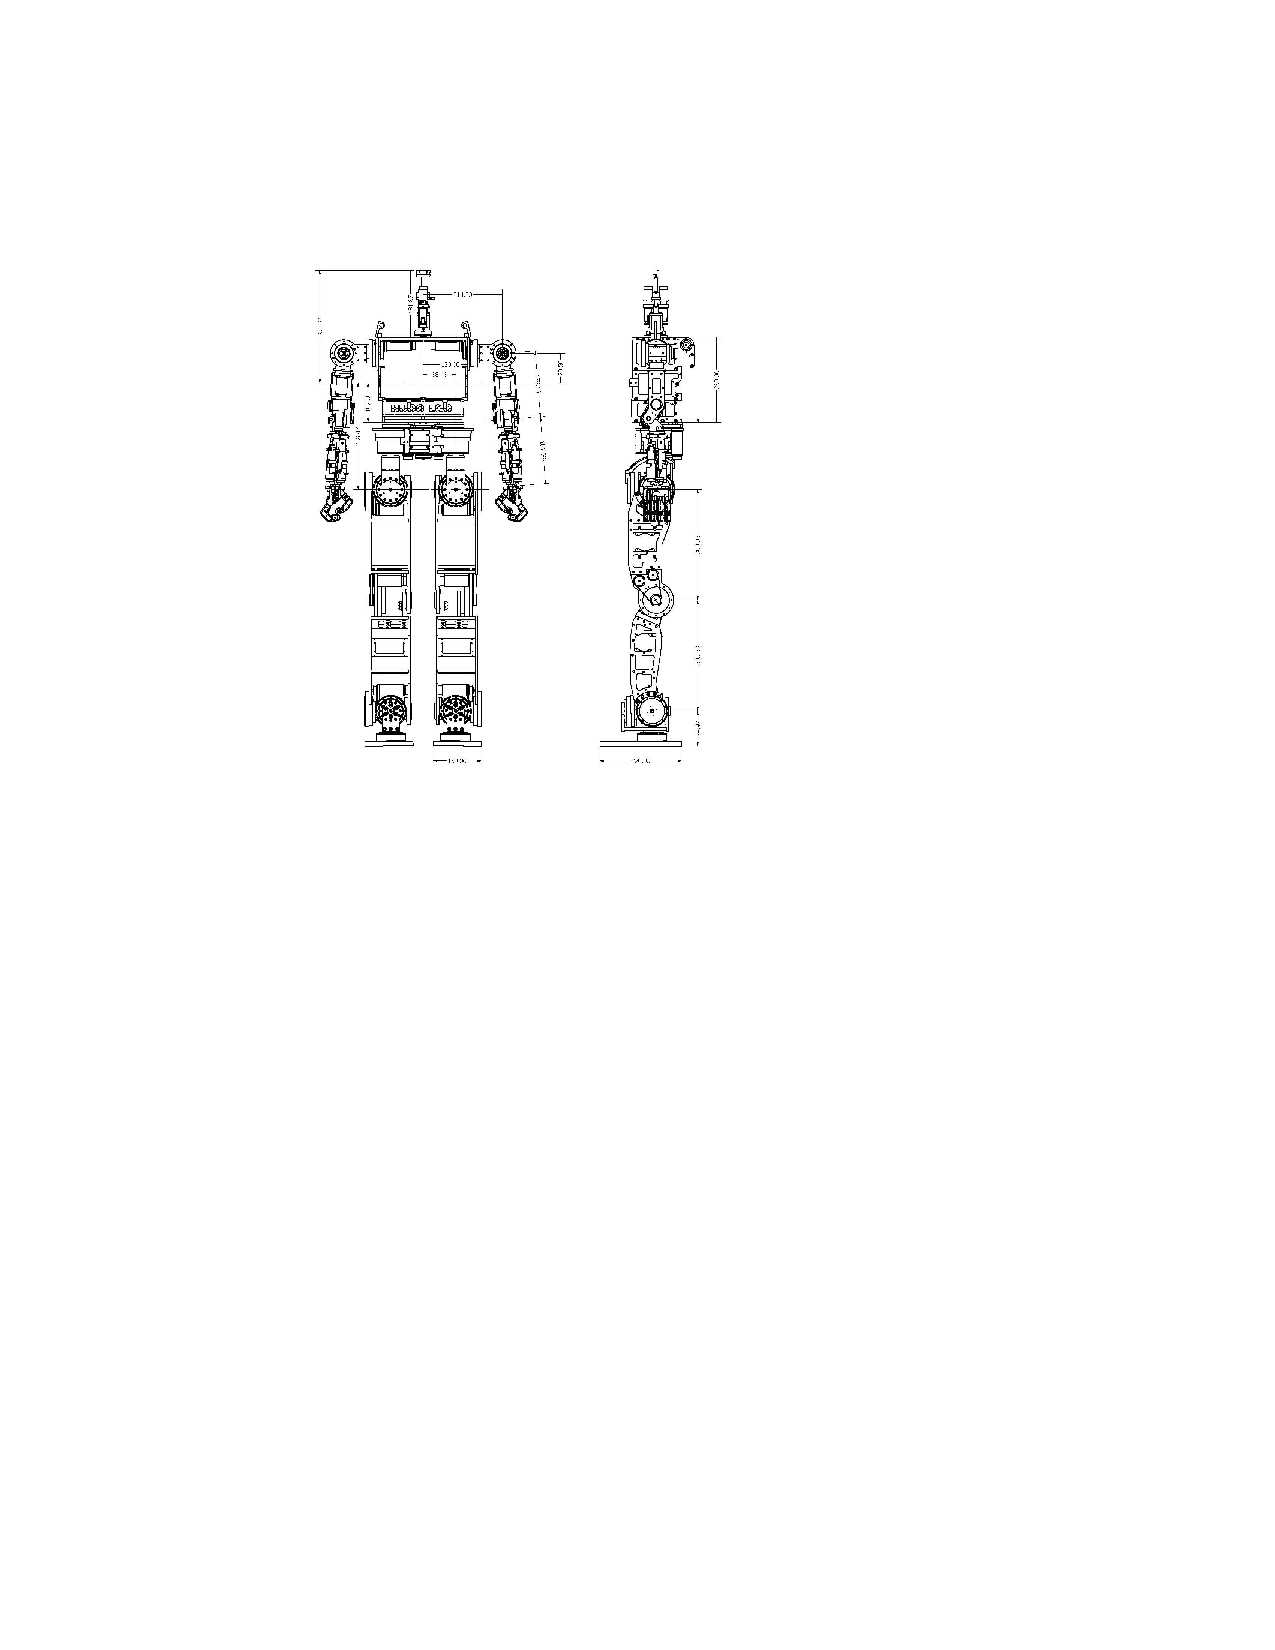
\includegraphics[width=1.0\columnwidth]{./pix/huboSkel.pdf}
  \caption{Hubo2 Plus platform: 38 DOF, 130 $cm$ tall full-size humanoid robot weighing 37 $kg$.}
  \label{fig:hubo}
\end{figure}



